\documentclass[letterpaper,twocolumn,10pt]{article}
\usepackage{usenix,graphicx}
\usepackage[colorlinks]{hyperref}
\begin{document}

%don't want date printed
\date{}

%make title bold and 14 pt font (Latex default is non-bold, 16 pt)
\title{\Large \bf Hash Integrity Checker:\protect\\An Integrity Checker for Downloads on your Browser}

\author{
{\rm Joshua Dawson}
\and
{\rm Peter Marheine}
\and
{\rm Frederico Rocha}
}

\maketitle

% Use the following at camera-ready time to suppress page numbers.
% Comment it out when you first submit the paper for review.
%\thispagestyle{empty}

\subsection*{Abstract}

Cryptographic hash functions are often used to verify the integrity of files downloaded from the internet, but are rarely published by distributors and rarely checked by users even when available. We present a browser extension and associated infrastructure for automating hash checking of all downloaded files, suitable for use no matter the availability of an official hash for verification and providing a dataset useful for following files over time on the greater Internet.

\section{Introduction}

Using cryptographic hash functions to compute file hashes is nothing new to the the Computer Security community; however, generating a Google Chrome extension to assist the user in verifying the authenticity of a file is novel. This inspired the development of Hash Integrity Checker. Hash Integrity Checker is a Google Chrome extension that assists the user in making informed decisions regarding the authenticity of a downloaded file. The extension computes the hash on a downloaded file and checks the hash against a database of known hashes to confirm that the download is what the user had intended.

The primary goal of Hash Integrity Checker is to provide the user with real time file verification feedback for any downloaded file. This ability to check file integrity should mitigate the risk of a user opening a file that has been corrupted with malware. Resulting in an overall safer computing environment for the user.

Existing browser extensions only allow the user to compute the hash for text input or a file they manually select from the local file-system. Once the hash is calculated and displayed to the user, the burden is then placed on the user to conduct the file authenticity check. This usually involves a visual comparison between the computed hash displayed on the screen and a hash provided by the web page serving the file. This may cause a problem if the web page serving the file does not display their own calculated hash for the file they are serving.

Our extension, Hash Integrity Checker, is different from previous extensions in that it computes the hash automatically for a downloaded file and then checks the hash against a database of known file hashes and then provides feedback to the user on the results of the check. This process is automated in such a way that it does not place any additional burden on the user. It provides feedback on the authenticity of a file but ultimately still allows the user to choose whether they trust that the file has not been tampered with.

\section{Related Work}

TODO Also, we have as related work ``Automating phishing website identification through deep MD5 matching"~\cite{Wardman}.

One of the challenges of creating a Google Chrome extension is navigating the Google Chrome extension security architecture. For the extension, we want to make sure we are requesting the correct permissions to achieve our design goals while ensuring that we are not using unnecessary permissions or requesting more access than is necessary for a permission. For example, when using the chrome.fileSystem API, and associated requested permission, is read access sufficient or does the application need write access as well? Previous researchers have detailed the security vulnerability involving the over-provisioning of permissions~\cite{180206}. For our extension we want to follow the guidelines set forth in their research to ensure we reduce the attack surface of our extension.

The Electronic Frontier Foundation's SSL Observatory~\cite{ssl-observatory} plays a role
similar to some aspects of the directory server in our system, where users of a browser
extension (HTTPS Everywhere~\cite{https-everywhere}) may opt to have the browser
submit observed SSL certificates to the Observatory. The SSL Observatory is available for
researchers to mine, of particular interest for investigating the reality of certificate authorities
on the web.

The browser plugins provided by VirusTotal~\cite{vtzilla,vtchromizer,vtexplorer} provide
methods for users to scan both web pages and files for malware. In all cases, however, the
user must specifically command the plugin to perform a scan so it is only useful if the user
is already cognizant of a malware threat. Our system works without any intervention
but only provides data, requiring that a user make a decision regarding whether they wish
to trust any given file. The data provided by our extension helps a user make a decision
whether they should trust that a file has not been tampered with, but cannot identify
malicious files distributed in ways that a user trusts.

\section{Design}

The design of our tool has gone through a number of implementation iterations, despite our design goals remaining fairly consistent through the design process. The following is a list of our design goals for this project:

\begin{enumerate}
\item There should be no restrictions placed on the type of file or the download location on the local file system.
\item The hashing of the file should automatically occur as soon as the file is downloaded without requiring additional input from the user after the download request is initiated.
\item The tool should verify the downloaded file for integrity and authenticity from a known file hash database.
\item The tool should provide feedback to the user based on the results of the file check.
\item The tool should not “quarantine” a file that is not found in the known file hash database but rather provide meaningful feedback to the user so that they can make an informed decision what to do with the downloaded file.
\end{enumerate}

Hash Integrity Checker is not a virus or malware scanning tool. By our specification Hash Integrity Checker is only conducting a file integrity and authenticity check by comparing the hash of the file against a known file hash database. The tool is not scanning the downloaded file for any malicious behavior as compared with extensions that are bundled with popular commercial anti-virus software. If a malicious file is found by a virus-scanner it is generally moved to a “quarantine” zone. It is the intent of Hash Integrity Checker to only hash the downloaded file and provide meaningful feedback to the user. It is left up to the user to decide, based upon the feedback, whether the downloaded file is the same file the user intended to download. It is still recommended to run anti-virus in conjunction with Hash Integrity Checker for a complete safe-computing solution.

\subsection{Implementation}

\begin{figure}
    \centering
    \fbox{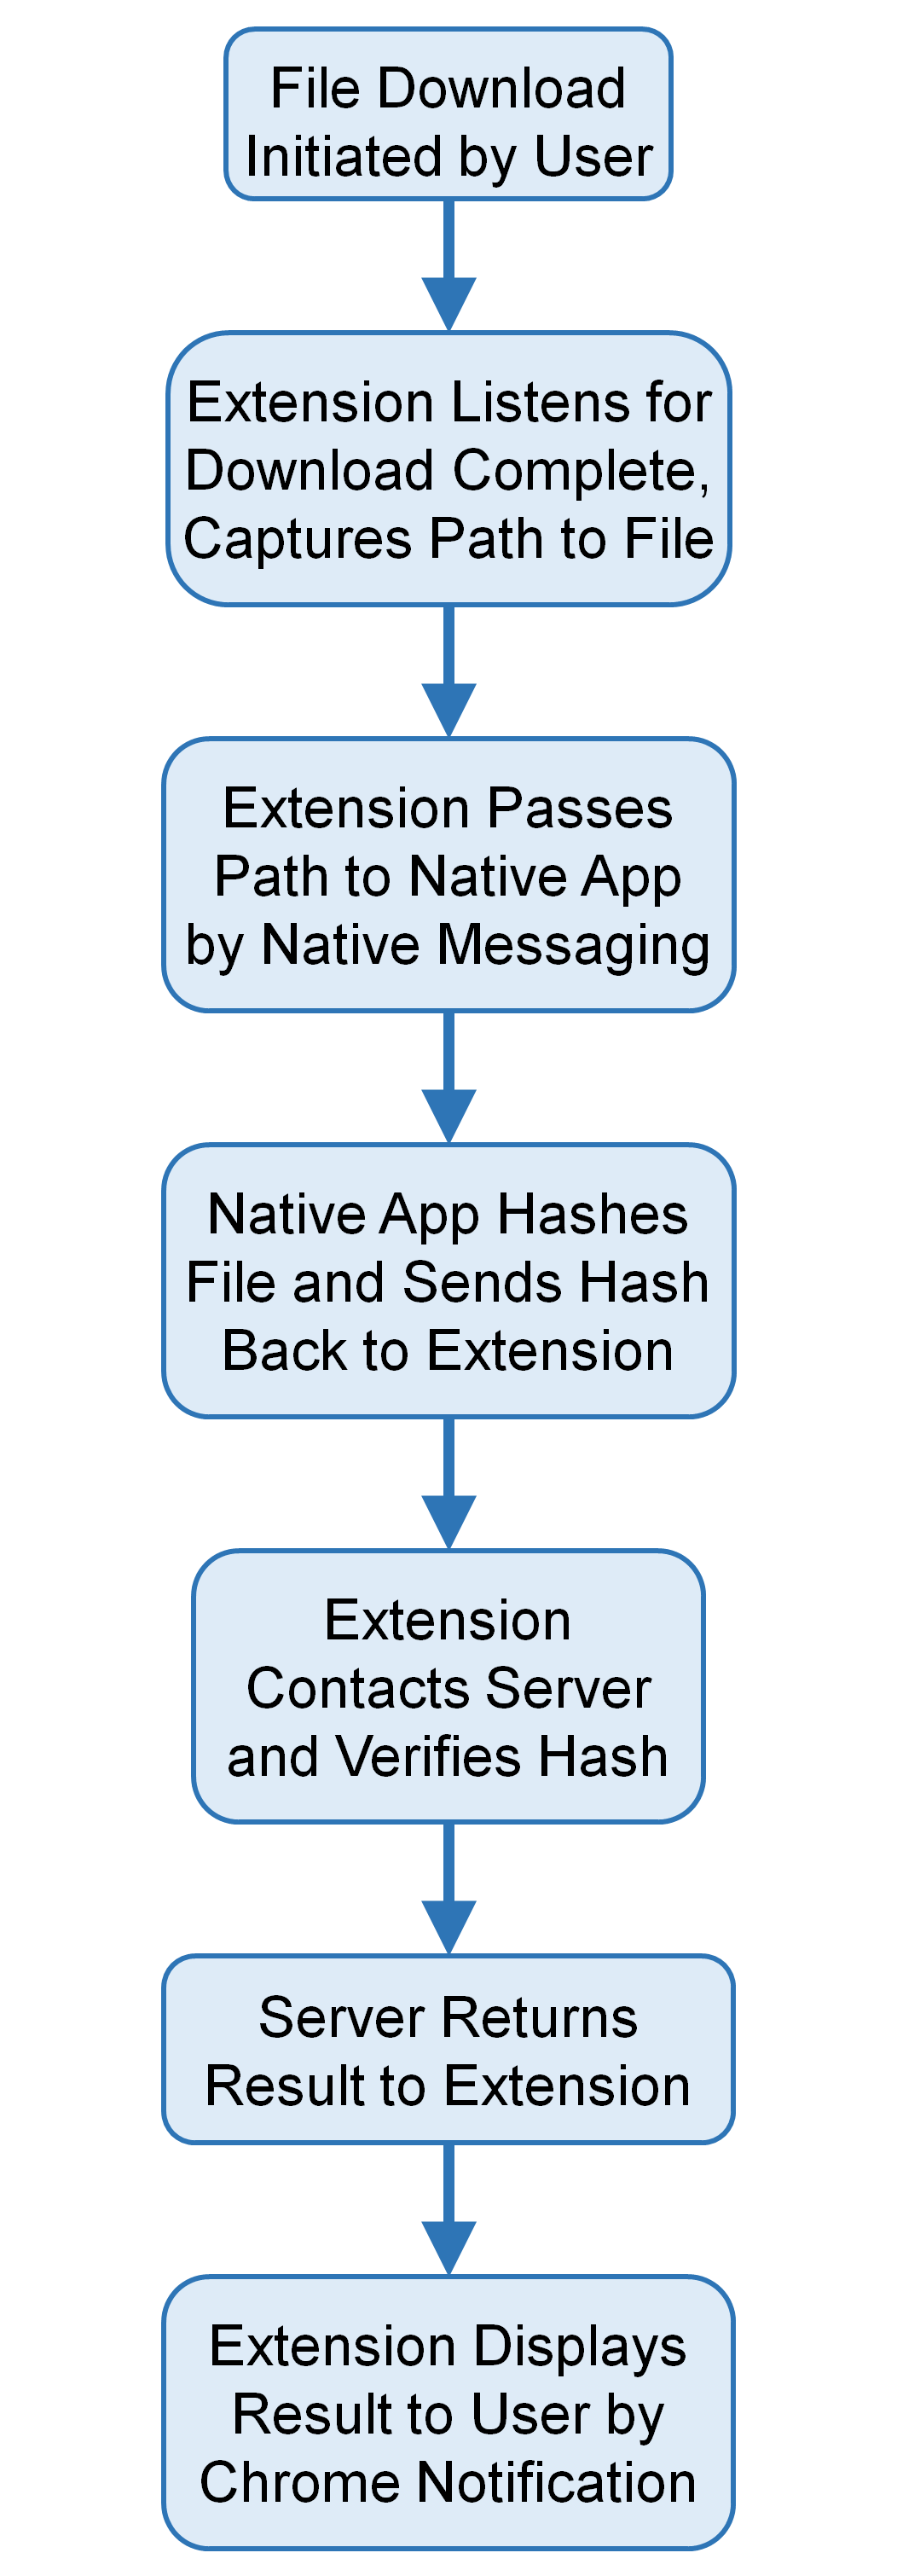
\includegraphics[width=0.5\columnwidth,keepaspectratio]{workflow-vertical.png}}
    \caption{Application Workflow}
    \label{fig:appflow}
\end{figure}

\begin{figure*}
    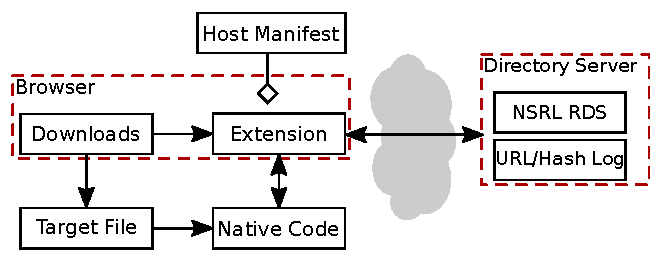
\includegraphics[width=\textwidth]{system.pdf}
    \caption{Logical dataflow through the system on download completion}
    \label{fig:sysflow}
\end{figure*}

Google Chrome's architecture has been the driving force for many of our design decisions
for the development of the tool. The browser's sandboxed design~\cite{chromium-security}
offers improved security guarantees relative to older methods for supporting extensions,
but also limits the capabilities available to most browser extensions.
For example, Google Chrome extensions are allowed access to the \texttt{chrome.downloads} API.
This allows the extension access to download events and can even fetch the download path on the
local file system for recently downloaded files. However, Google Chrome extensions do not have
direct access to the filesystem. This means that even though the extension can know
the path to the downloaded file on the local filesystem, it is not allowed to have any interaction with
the downloaded file.

The first iteration of our design included just a single Chrome extension. We managed to skirt the
issue of not having access to the \texttt{chrome.fileSystem} API by forcing the user to download
any file to a downloads folder located in the install folder of the extension. This solves the problem
of not having access to the \texttt{chrome.fileSystem} API because extensions do have access to
files that are located in their own install directory. Obviously this conflicts with our first design goal.
By forcing the user to download to a specific folder it ruins the flexibility and usability of the extension.
Furthermore, the extension’s install directory is only available if the extension is loaded as an unpacked
extension, which requires the user to load the unpacked extension in developer mode and precludes
the option to deploy our extension to the Chrome Web Store. The restrictions placed by Google on
the accessibility of a Chrome extension’s use of certain APIs meant we would have to explore another
route to meet this design challenge.

The second iteration of our design utilized a combination of a Chrome extension and a Chrome app.
The Chrome extension had access to the \texttt{chrome.downloads} API, for which the app does not,
and the Chrome app had access to the \texttt{chrome.fileSystem} API, for which the extension does not.
By using the combination of the extension and the app we were hoping to overcome the challenges of the
sandboxed environment place on each component. The extension would listen for the file download to
complete and then it would wake up the app and pass a message to the application containing the
path to the downloaded file. The app would receive the message and display it as a prompt to the user.

Even though Chrome apps have access to the \texttt{chrome.fileSystem} API, they require a user
action to be able to access the local filesystem. By design this is to prevent malicious apps from
modifying files on the local filesystem without the user’s consent. The user action that is defined
in the documentation for the API generally relates to an open file dialog that allows the user to select
a file. This action of physically selecting a file demonstrates that the user is giving permission to the
application to access the local filesystem. By requiring the user to open the file they just downloaded,
this iteration of our design is comparable to other hashing applications available in the Chrome
Web Store which require user intervention. 

Our app could be used in a standalone fashion if
the user chooses not to install the extension, but this design does not satisfy the design goal
that files should be hashed automatically on download completion without user intervention.
Originally we had desired to incorporate the entire tool as an extension; however, we learned
over time that it was going to require native messaging with a native application to achieve all
of our design goals.


The final iteration of our tool utilizes native messaging between our Chrome extension and a
native application as illustrated in \autoref{fig:sysflow}. The Chrome extension receives the download completed event from the
\texttt{chrome.downloads} API, and sends a message containing the path of the file in question
to the native application. The native application then computes the hash of the file and
sends a message back to the extension with the hash digests. The overall workflow of the application is depicted in \autoref{fig:appflow}.

With the information available to it and hash digests computed by the native application,
the extension may perform whatever processing is desired to determine whether the
downloaded file is consistent with what was expected.
The extension then opens a Chrome notification window to display its conclusions.
This final iteration achieves all of our design goals. Our Google Chrome extension allows
the user to seamlessly download any file from any website to any location on the local
filesystem. The hash is calculated and verified against a known file hash database and
the feedback results are relayed to the user via a Chrome notification window, examples
of which are shown in \autoref{fig:ss-none} and \autoref{fig:ss-match}.

Use of a native component running outside the browser requires two components:
a program which can be executed natively by the host operating system, and a manifest
declaring to the browser where that program may be found and which extension(s) are
allowed to communicate with it. Since these components cannot be packaged and installed
as part of a browser extension package, the extension must be installed through the
system's usual methods.

The binary component is written in standard C, with components from mbed TLS~\cite{mbedtls}
for computing cryptographic hashes. A platform-appropriate installer is generated containing
this program and a manifest file, which when invoked by a user will install the binary component
and manifest file for the extension, and can trigger installation of the browser component.
This process has not been implemented fully because automating installation of components
in the browser requires that they be published on the Chrome Web Store (for security reasons),
which we have not done.

\subsection{Validity heuristics}

The ability to compute hashes of downloaded files automatically is often of limited utility,
because users lack the information to make a decision regarding the validity of the
resultant hash. A simple heuristic exists in our current implementation, with the capability
to add more with relatively little effort.

In some cases, digests are available from the publisher; sometimes directly on the web page
which triggered the download, or other times in files next to the downloaded file on the
originating server. The information regarding these sources is available to the extension
code, so digests in these locations can be discovered through probing. Though we have not
implemented this function, a functioning design might specify a series of rules to identify
published digests, each of which matches certain properties of the source URL and
contents of the referring page.

For example, some file hosts publish checksums directly on the download pages. The
extension could match the referring URL against those matching a known host, then
scrape the referring page to retrieve the checksum's value. In cases where no host-specific
rules match, the extension may attempt to retrieve the directory containing the
downloaded file and search for files with names commonly used for checksums. For
example, a download of \texttt{https://example.com/linux/linux.iso} might prompt the
extension to search for checksums contained in
\texttt{https://example.com/linux/sha1sums.txt}.

If none of these heuristics are successful in finding published hashes for a file (as is
the case in our current implementation), it may (at the user's option) contact
a ``directory server'' in hopes of finding information about the downloaded file.
The directory server's operation and features are discussed in \autoref{sec:dirserver}.

\begin{figure}
    \fbox{
\includegraphics[width=\columnwidth]{hash-notify-matched.png}}
    \caption{Message when no matches exist}
    \label{fig:ss-none}
\end{figure}

\begin{figure}
    \fbox{
\includegraphics[width=\columnwidth]{hash-notify-none.png}}
    \caption{Message when matching files exist}
    \label{fig:ss-match}
\end{figure}

\section{Directory Server}
\label{sec:dirserver}

An integral part of our design was to have the directory server be a separate black box component to our extension. Our extension should be able to send the hash calculated by the native application, as well as any other pertinent file identification information such as file name and download URL, to the directory server. The directory server would then check the transferred arguments against its internal database and produce usable feedback to send back to the extension to notify the user. This model allows the user to decide what directory server is most trustworthy for their particular application. In this section we provide two examples of directory servers that were used in the development of our application.

\subsection{VirusTotal Directory Server}

The first directory server we linked to was the VirusTotal public API. VirusTotal is a free online service that allows a user to upload a file and have it checked against the output obtained from multiple antivirus products. VirusTotal itself is not a standalone antivirus solution, it considers itself to be an information aggregator from those commercial products~\cite{vtabout}. One benefit for our application is that VirusTotal keeps a record of the associated hashes of files that are uploaded to their system to be checked for malware. This provides us with an easy proof of concept solution to provide feedback results for our extension. This allows us to test our extension against a working database that is already preloaded with a large sample of file hashes.

One of the methods for looking up a file using the VirusTotal public API is by sending VirusTotal the SHA-256 hash of the file. This method is used in our application to verify if the user's downloaded file is contained in the VirusTotal database. We chose this method since our native application has already calculated the hash of the file before connecting to a directory server. If the file is in the database we return the file name and detection results from VirusTotal back to the extension. The extension then creates a Chrome notification box that displays the results to the user. If the user clicks on the Chrome notification box the VirusTotal web page associated with the hash of their downloaded file is automatically opened so the user can see the full VirusTotal results. If the file hash is not in the VirusTotal database the Chrome notification displays the SHA-256 hash along with a message notifying the user that the file hash is not in the database. Whether the file hash is contained in the database or not it is left up to the user to decide if they trust the integrity of the file. The hash is displayed if the user wants to seek a different opinion from an alternate file hashing service or if they are able to make a comparison with a hash provided by another source; for example, a hash provided directly by the serving web page for the file.

One of the drawbacks to using the VirusTotal directory server is that you have to have trust in VirusTotal to trust the results. Also since VirusTotal is mainly a malware checker, and not primarily focused on file integrity, it is still susceptible to a poisoning attack. If an attacker uploads their own malicious file to the VirusTotal server, that is not currently detectable by the commercial malware scanner VirusTotal uses, VirusTotal will just add that file information into their database. Then if a user downloads the file from a malicious hosting website using our extension they may get a false sense of security because the file was found in the VirusTotal database. VirusTotal tries to counter this attack by having a community voting option. For any VirusTotal results web page there is an option for any user to vote if the file is suspected to be malicious or not. The voting system is supposed to reassure the user and assist in making a decision about the file and move trust away from VirusTotal and more towards trust in the group consensus ~\cite{GroupPolarization}. This is also easily attacked because anonymous votes are allowed by the voting system; therefore, a diligent attacker would ensure there is numerous thumbs up votes for their malicious file.

This complication of determining whether a file is malicious or not is one of the reasons Hash Integrity Checker focuses only on providing feedback about the file integrity. In the case above about downloading a malicious file from a malicious web server, Hash Integrity Checker should only confirm that the file is indeed the file you intended to download. It is still left up to the user to use other tools, like a malware scanner, to determine if the file is malicious.

\subsection{Custom Directory Server}

Our directory server provides access to a database of observed files, including their
source and hash digests, over an HTTP API suitable for use by the browser extension.
It encapsulates two logical data sources: the NSRL RDS and collected files.

The NSRL RDS~\cite{nsrl-rds} is a database of publicly-distributed software maintained by the
National Institute of Standards and Technology, including the files contained within each
of those software products, describing approximately 42 million files at the time of this
writing. The directory server has a partial copy of the RDS, usable to determine
whether a given file (identified by name and hashes) is known to exist in the RDS
but not able to indicate what the possible sources of the file are.

The collected files database is both readable and writable in an append-only mode
(whereas the RDS is read-only), and receives information from the browser extension
when enabled by the user (submission is disabled by default to prevent unexpected
information disclosure) regarding the source, hash digests, and name of downloaded
files, including the time at which a given file was seen.

The two datasets stored by the directory server are searchable over the HTTP
API, so the browser extension may search for known files which match ones
that have been seen before. In our current implementation, the browser extension
searches for entries with the same source URL. Matching files (if any) are
treated as a partial consensus among previously-observed instances of the file,
and the overall agreement is reported to the user as illustrated in \autoref{fig:ss-match}
and \autoref{fig:ss-none}.

Though the current use of the directory server is limited, it is possible for more
sophisticated analyses to be built on this data set. For example, it may be
useful to weight more recent reports higher than older ones, recognizing
that the contents (and thus hashes) of any given file may change over time.
Changes that have been corroborated over longer periods of time are less
likely to be the unexpected, whereas a sudden change in a file's contents may indicate
an attack or integrity failure.

\section{Threat Model}

This section needs revision and fleshing out.

What does hash checking guard against? Inadvertent corruption, MITM-based tampering, compromised servers (tampering again). We protect against corruption when official hashes are published, and can sometimes detect either flavor of tampering depending on time-related properties (how long it’s been there, how popular the file is).

In case of a changed file on a server, if the published hashes are not modified the difference will be noticed. If published hashes are updated (suggesting a savvy attacker or actual update by the publisher), the difference between records in the directory and published hashes will (could) be noted. The user must still decide whether they trust the change.

Attackers might try to poison the directory. Mitigated somewhat by making
it possible to use a custom directory server, so eg an organization running a large private
network can't have a private directory attacked easily.

\section{Discussion}

This section needs revision and fleshing out.

Few users ever take advantage of published hashes when downloading files, and those who do usually only verify hashes on certain classes of files (particularly disk images). Built-in integrity checks such as checksums embedded in many kinds of archive files offer some confidence that a file has not been inadvertently corrupted, but are generally not robust against malicious tampering.

In many cases checksums (or cryptographic hashes) are not even published by the publisher of a file, or are not provided via the distribution medium such as a public file hosting web site. Our system provides a back-channel for verification of files, provided sufficient data.

Code signing systems can provide stronger protections against tampering in-transit, such as Authenticode~\cite{Authenticode} on Windows and Gatekeeper ~\cite{Gatekeeper} on OS X, both of which provide strong cryptographic guarantees regarding the authenticity for application packages. Both of these systems are limited, however, in that they require the user put trust in a third party (a certificate authority or Apple, respectively) that malicious parties cannot resign modified applications after tampering with them.

A sufficiently motivated  and savvy attacker could simply submit hashes of a tampered file to the directory to attempt to get users to accept that as the true hash. Such tampering might be detectable, but our current design of the system does not include any such functionality. At the directory, it is also possible to attempt to reject invalid hashes via any number of methods. If the methods applied to reject certain reports are public it becomes easier to work around them given a motivated attacker, a weakness of the open architecture of the system. It would thus be advantageous not to expose the details of rejections (make the API always report success). It is likely possible to implement a sort of trust system for clients reporting file metadata to the directory, which would also help mitigate the risk of directory-poisoning attacks.

The extension does however allow users to run their own directory server and specify where it can be reached. Running a non-public directory server is an effective defense against directory attacks, since an attacker capable of reaching a private directory is likely also capable of directly compromising a target without relying on tampering with downloaded files.

The directory server is potentially interesting for study of how often files are updated, possibly detecting tampering, measuring error rates, other things.

\section{Limitations}

This section needs revision and fleshing out.

Hashing performance may be poor due to choice of native hash implementations (from mbedTLS, which is easily portable but not particularly optimized).

Setup is not as trivial as we would have liked. Requires installation of a native component, and actually providing a useful installer requires publishing the extension on the Chrome Web Store, which we have not done because it costs money.

Currently only supports Google Chrome (more generally, Chromium derivatives). There is no technical reason we can't support other browsers (Firefox, IE/Edge), but we chose to focus effort on only one implementation.

Currently depends on  user-submitted files for the most part. We could seed the database somehow (like scraping lots of the web for files and hashing them, assuming our seeding process is not tampered with), but that’s not great. We also assume honest reports, as noted in the discussion.

\section{Evaluation}
Admittedly the final result of our tool is not exactly what we had originally set out to accomplish. We had wanted to create a standalone Google Chrome extension that would allow the user to download a file, compute the hash, and give feedback about the authenticity of the file to the user. As we have discussed before, the feasibility of being able to accomplish all of this within a Chrome extension alone does not appear to be possible by design of the Chrome sandboxed architecture. Through additional research into Chrome extension implementation we were able to create a Chrome extension that uses native messaging between our extension and a native application to achieve all of our design goals.

For this project we would have preferred to do a user study to measure the viability of using Hash Integrity Checker on a consistent basis. Due to the compressed timeline of this project we were not able to implement the final product with enough time to execute a formal user study. We were able to do an internal test of our system by having the extension installed and running on our machines.

For three weeks we were able to test our extension in a live environment. The extension was installed for the Google Chrome browser and was used with every download during that time period as part of our regular web browsing behavior. As expected, and by design, the extension was actually useful for verifying the integrity of downloaded files. The feedback provided in the Chrome notification box allowed us to make an informed decision whether we wanted to accept or discard the downloaded file. The extension did not cause a distraction or reduction in performance to the overall web browsing experience. We leave deploying Hash Integrity Checker on a larger scale, and conducting a formal study of the user experience with our extension, as future work.

\section{Future Work}

This section needs content.

{\footnotesize \bibliographystyle{acm}
\bibliography{bibliography}}

\end{document}